
\chapter{The Serre Equations}
\label{chp:Serreeqns}
The Serre equations are a system of partial differential equations that describe the free-surface waves of fluids. They are an approximation to the Euler equations \cite{Euler-1755-274}; describing waves in shallow water when the characteristic depth of the water $h_0$ is far smaller than the characteristic wavelength of the waves $\lambda_0$ so that the shallowness parameter $ \sigma = h_0 / \lambda_0  \ll 1 $. Typically, water is considered to be shallow when $\sigma  \le  1/ 20$ \cite{Sorenson-2006}.  

The Serre equations for one-dimensional flows over horizontal beds were first derived by \citet{Serre-F-1953-857} using asymptotic expansion then later derived using depth integration by \citet{Su-Gardener-1969-536}; they are equivalent to the Green-Naghdi equations \cite{Green-Naghdi-1976-237} derived using the theory of directed fluid sheets. The Serre equations were then extended to spatially varying bathymetry by \citet{Seabra-Santos-etal-1987-117}. 

The Serre equations are fully nonlinear and thus applicable across the entire range of characteristic wave amplitudes $a_0$ which are usually summarised using the nonlinearity parameter $\epsilon = a_0 / h_0$. The fluid described by the Serre equations possesses a non hydrostatic pressure distribution and thus is dispersive in nature, as are real fluids. Furthermore, the dispersion relationship of linear waves of the Serre equations well approximates the linear wave theory for the Euler equations \cite{Barthelemy-2004-315}. For these reasons the Serre equations are considered one of the best approximate water wave models \cite{Bonneton-Lannes-2009-16601,Bonneton-etal-2011-1479}. 

In this chapter we present the one-dimensional Serre equations and a reformulation of these equations into conservation law form. We then present the relevant properties of the Serre equations that will be used to assess the validity of the developed numerical methods, ending with the contribution of my research to the known properties of the Serre equations; the evolution of steep gradients in the free-surface. 

\section{The Equations}
%[!]-----[!] DISPERSION!!!!!
%full nonlineariy, good approximation to Euler equations up to wave breaking
In this thesis we take the Serre equations as derived from depth-integration approach \cite{Su-Gardener-1969-536,Seabra-Santos-etal-1987-117}. Given the extent of the literature already available for the derivation of these equations we will only introduce the relevant quantities and present the equations. Under the depth-integration approach the one-dimensional Serre equations describe the behaviour of unsteady free surface fluid flow for an inviscid fluid with constant density $\rho$, neglecting wave-breaking and bottom friction. The primitive variables are the height $h(x,t)$ of the free surface above a stationary bed profile given by $b(x)$ and the depth average horizontal velocity $u(x,t)$ which are all demonstrated in Figure \ref{fig:WaterModel}. Additionally we define the stage $w(x,t) = h(x,t) + b(x)$ which gives the absolute location of the free surface. The derivation is similar to that of the Shallow Water Wave Equations (SWWE) \cite{Liggett-1994}, except for the Serre equations the vertical velocity $v(x,z,t)$ varies linearly with depth and is given by \cite{Zoppou-2014}
\begin{equation}
v(x,z,t) = u \frac{\partial b}{\partial x} - (z - b) \frac{\partial u}{\partial x}.
\label{eqn:VertVelSerre}
\end{equation}
Unlike the SWWE the vertical velocity of the Serre equations is not zero throughout the depth of water consequently the Serre equations possess a non-hydrostatic pressure distribution
\begin{equation}
\label{eqn:SerrePress}
 p(x,z,t) = \underbrace{g \rho \left(h + b - z\right)} + \rho \left(h + b - z\right) \Psi + \frac{1}{2} \rho \left(h^2 - \left[z - b \right]^2\right) {\Phi }
\end{equation} 
where
\begin{subequations}
	\begin{align}
	{ \Psi }  &= \dfrac{\partial b}{\partial x}\left(\dfrac{\partial u}{\partial t} + u\dfrac{\partial u}{\partial x} \right)  + u^2\dfrac{\partial^2 b}{\partial x^2}, \label{eqn:SerreeqnPsi} \\ \nonumber \\
	{ \Phi }  &= \dfrac{\partial u }{\partial x} \dfrac{\partial u}{\partial x} -u \dfrac{\partial^2 u}{\partial x^2}  - \dfrac{\partial^2 u}{\partial x \partial t} . \label{eqn:SerreeqnPhi} 
	\end{align}
	\label{eqn:FullSerreNonConVarDef}
\end{subequations}
\begin{figure}
	\centering
	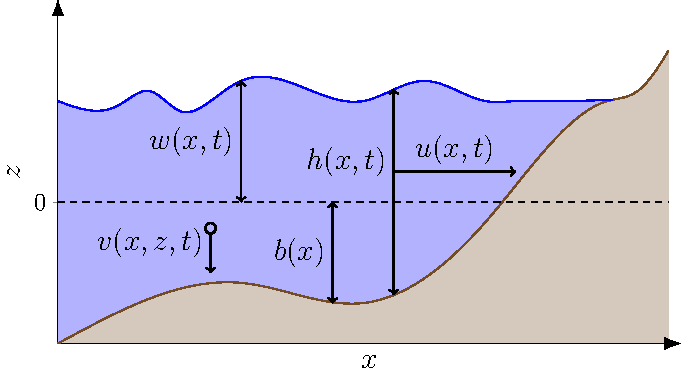
\includegraphics[width=0.8\textwidth]{./chp2/figures/SerreModel.pdf}
	\caption{Diagram demonstrating the quantities used to describe the fluid (\squareF{blue}) and the bed (\squareF{brown!80!black}) for the Serre equations.}
	\label{fig:WaterModel}
\end{figure}
By depth integrating the Euler equations \cite{Su-Gardener-1969-536,Zoppou-2014} with a no-slip condition at the bed, a free surface condition at the free surface,the vertical velocity relation \eqref{eqn:VertVelSerre} and the pressure distribution \eqref{eqn:SerrePress} we obtain the depth integrated approximation of the conservation of mass and momentum equations
\begin{subequations}
	\begin{align}
	&\frac{\partial h}{\partial t} + \dfrac{\partial (uh)}{\partial x} = 0,  \label{eqn:FullSerreNonConMass} \\ \nonumber \\
	&\dfrac{\partial (uh)}{\partial t} + \dfrac{\partial}{\partial x} \left ( u^2h + \dfrac{gh^2}{2} + \dfrac{h^2}{2}{\Psi} + \dfrac{h^3}{3}{ \Phi }  \right )  +  \dfrac{\partial b}{\partial x} \left (gh +   h \Psi + \dfrac{h^2}{2}{ \Phi }  \right ) = 0	\label{eqn:FullSerreNonConMome}
	\end{align}
	\label{eqn:FullSerreNonCon}
\end{subequations}
When $\Phi = \Psi = 0$ the Serre equations reduce to the SWWE where the vertical velocity is zero, so that only the hydrostatic part of the pressure is present and there is no dispersion. 

Due to the presence of the $\Phi$ and $\Psi$ terms the Serre equations are more difficult to solve analytically and numerically than the SWWE. The primary reason for this is that whilst the SWWE are hyperbolic the Serre equations are neither hyperbolic nor parabolic. Furthermore, the Serre equations are not in conservation law form due to the presence of temporal derivatives in $\Phi$ and $\Psi$, although they are derived from conservation equations. 

For a horizontal bed $\partial b / \partial x = 0$, $\Psi = 0$ and so the Serre equations reduce to
\begin{subequations}
	\label{eqn:FullSerreNonConHorizbed}
	\begin{align}
	\label{eqn:FullSerreNonConMassHorizbed}
	&\frac{\partial h}{\partial t} + \dfrac{\partial (uh)}{\partial x} = 0, \\ \nonumber \\
	\label{eqn:FullSerreNonConMomeHorizbed}
	&\dfrac{\partial (uh)}{\partial t} + \dfrac{\partial}{\partial x} \left ( u^2h + \dfrac{gh^2}{2} + \dfrac{h^3}{3}{ \Phi }  \right ) = 0.
	\end{align}
\end{subequations}	
For horizontal beds the Serre equations are more challenging to solve analytically and numerically than the SWWE. 

\subsection{Alternative form of the Serre Equations}
A major hurdle for developing numerical methods for the Serre equations is the presence of the mixed temporal and spatial derivative in $\Phi$ and $\Psi$ \eqref{eqn:FullSerreNonConVarDef}. By rewriting the Serre equations and introducing a new conserved quantity $G$ \cite{Hank-etal-2010-2034,Zoppou-2014,Li-2014-169}, the mixed temporal and spatial derivatives can be removed and the Serre equations can be written in conservation law form with a source term. The introduced conserved quantity is
\begin{equation}
\label{defn:SerreEqnConservedQuantity1}
G =  h {u} \left(1 + \frac{\partial h}{\partial x}\frac{\partial b}{\partial x} + \frac{1}{2}h\frac{\partial^2 b}{\partial x^2} + \left[\frac{\partial b}{\partial x}\right]^2 \right) - \frac{\partial}{\partial x}\left(\frac{1}{3}h^3  \frac{\partial {u}}{\partial x}\right).
\end{equation}
The Serre equations \eqref{eqn:FullSerreNonCon} can then rewritten as conservation laws with a source term for the conserved variables $h$ and $G$
\begin{subequations}
	\label{eqn:FullSerreCon}
	\begin{align}
	& \frac{\partial h}{\partial t} + \dfrac{\partial (uh)}{\partial x} = 0 ,\label{eqn:FullSerreConMass}  \\ \nonumber \\
	\begin{split}
	\label{eqn:Serreconsconmom}
		\frac{\partial G}{\partial t}  + \frac{\partial}{\partial x} \left( {u} G + \frac{gh^2}{2} - \frac{2}{3}h^3 \left[\frac{\partial {u}}{\partial x}\right]^2 + h^2 {u}\frac{\partial {u}}{\partial x}\frac{\partial b}{\partial x} \right) \\ \\ + \frac{1}{2}h^2 {u} \frac{\partial {u}}{\partial x} \frac{\partial^2 b}{\partial x^2}  - h {u}^2\frac{\partial b}{\partial x}\frac{\partial^2 b}{\partial x^2} + gh\frac{\partial b}{\partial x} = 0.
	\end{split}
	\end{align}
\end{subequations}
The conserved quantity $G$ resembles $h$ multiplied by the irrotationality \cite{Choi-Camassa-1999-1,Carter-Cienfuegos-2011-259}.

This conservation law form makes the Serre equations well suited to be numerically solved using a finite volume method for the conservation of mass and $G$ equations, provided one can solve for $u$ given $h$ and $G$.

For a horizontal bed $\partial b / \partial x = 0$ the conservation law form of the Serre equations using the new quantity $G$ is
\begin{subequations}
	\label{eqn:FullSerreConHorizBed}
	\begin{align}
	&\frac{\partial h}{\partial t} + \dfrac{\partial (uh)}{\partial x} = 0, \label{eqn:FullSerreConMassHorizBed} \\  \nonumber \\
	&\frac{\partial G}{\partial t}   + \frac{\partial}{\partial x} \left( {u} G + \frac{gh^2}{2} - \frac{2}{3}h^3 \left[\frac{\partial {u}}{\partial x}\right]^2 \right) = 0 , \label{eqn:SerreconsconmomHorizBed}\\ \nonumber \\
	&G =  h {u}  - \frac{\partial}{\partial x}\left(\frac{1}{3}h^3  \frac{\partial {u}}{\partial x}\right). \label{defn:SerreEqnConservedQuantity1HorizBed}
	\end{align}
\end{subequations}


\section{Properties of the Serre Equations}
The Serre equations possess a number of properties that can be used to assess the veracity of numerical methods. If a numerical method approximates the Serre equations accurately then the properties of the numerical method should approximate the properties of the Serre equations. In this thesis the conservation properties, dispersion properties and analytic solutions of the Serre are employed and so are presented here. 

To complement the available analytic solutions, the Serre equations are modified to force certain analytic solutions using a source term, which are called forced solutions. These forced solutions will be used to assess the validity of the numerical methods for a wider array of flow scenarios then possible given the limited number of analytic solutions for the Serre equations.

Finally the results of \citet{Pitt-2017-1725} for the behaviour of the Serre equations in the presence of steep gradients are presented. These results demonstrate that the developed numerical method is robust in the presence of steep gradients; one of the main objectives of the Thesis. 

\subsection{Conservation Properties}
Conservation of a quantity means that in a closed system the total amount of a quantity $q$ remains constant in time.
\begin{defn}
	\label{defn:TotalAmmountab}
	The total amount of a quantity $q$ in a system occurring on the interval $[a,b]$ at time $t$ is
	\begin{equation*}
	\mathcal{C}_q(t) = \int_{a}^{b} q(x,t)\, dx.
	\end{equation*}
\end{defn}
Conservation of a quantity $q$ means that $\mathcal{C}_{q}(0) = \mathcal{C}_{q}(t)$ for all $t$. Given that the Serre equations \eqref{eqn:FullSerreNonCon} are conservation equations for mass and momentum and that the conservation of momentum equation can be rewritten as a conservation equation for $G$ \eqref{eqn:FullSerreCon}, the Serre equations conserve all these quantities. Additionally the Green-Naghdi equations \cite{Green-Naghdi-1976-237} which are equivalent to the Serre equations for one dimensional flows were derived by conserving the energy
\begin{equation}
	\mathcal{H}(x,t) = \frac{1}{2} \left( gh\left(h + 2b\right) + hu^2  + \frac{h^3}{3} \left[\frac{\partial u}{\partial x}\right]^2 + u^2h\left[\frac{\partial b}{\partial x}\right]^2 - uh^2 \frac{\partial u}{\partial x} \frac{\partial b}{\partial x}  \right).
	\label{eqn:Hamildef}
\end{equation}
Therefore, the one dimensional Serre equations should also conserve $\mathcal{H}$. The energy $\mathcal{H}$ is the sum of the gravitational potential energy, the horizontal kinetic energy and the vertical kinetic energy which integrated over the depth of water are
\begin{align*}
& \frac{1}{2}\int_{b}^{h +b} gz \; dx = \frac{1}{2}gh\left(h + 2b\right), \\
& \frac{1}{2}\int_{b}^{h +b} u^2 \; dx = \frac{1}{2}hu^2, \\
& \frac{1}{2}\int_{b}^{h +b} v^2 \; dx = \frac{1}{2} \left(\frac{h^3}{3} \left[\frac{\partial u}{\partial x}\right]^2 + u^2h\left[\frac{\partial b}{\partial x}\right]^2 - uh^2 \frac{\partial u}{\partial x} \frac{\partial b}{\partial x} \right),
\end{align*}
respectively. Where the vertical velocity $v$ in the Serre equations is given by \eqref{eqn:VertVelSerre}. For horizontal beds $\mathcal{H}$ is the Hamiltonian of the Serre equations \cite{Li-Y-2002}.
 
For the system to be closed the flux terms of the conservation of mass and momentum equations at the boundaries must cancel and the integral of the source term over the domain must be zero.

\subsection{Dispersion Properties}
The dispersion properties of wave equations are primarily studied through linearising the equations, assuming periodic wave solutions and then deriving a relationship between the frequency $\omega$ and the wave number $k$ of these solutions. For the Serre equations the dispersion relation \cite{Li-2014-169} is
\begin{equation}
\label{eqn:DispersionRelation}
\omega^\pm = Uk \pm k \sqrt{gH} \sqrt{\frac{3}{\left(kH\right)^2 + 3}}
\end{equation}
where $U$ and $H$ are the mean velocity and height of the fluid respectively and the subscript $\pm$ denotes the positive and negative branches of the dispersion relation. \citet{Barthelemy-2004-315} compared this dispersion relation to that of the linear theory of water waves and demonstrated its utility when $k$ is small. However, when $k$ is large the difference between the dispersion relation of the Serre equations and that of water wave theory increases. The dispersion relation of the Serre equations can be modified by introducing terms to reduce this difference \cite{Barthelemy-2004-315}, but such modifications are beyond the scope of this thesis.


From the dispersion relation \eqref{eqn:DispersionRelation} the phase velocity $v_p^\pm = \omega^\pm / k$  and the group velocity $v_g^\pm = \partial \omega^\pm / \partial  k$ can be written in terms of the wave number as
\begin{subequations}
	\label{eqn:WaveVelocities}
	\begin{equation}
	\label{eqn:WaveVelocitiesPhase}
	v_p^\pm = U \pm \sqrt{gH}\sqrt{\frac{3}{\left(kH\right)^2 + 3}},
	\end{equation}
	\begin{equation}
	\label{eqn:WaveVelocitiesGroup}
	v_g^\pm = U \pm \sqrt{gH} \left(\sqrt{\frac{3}{\left(kH\right)^2 + 3}} \mp \left(kH\right)^2 \sqrt{\frac{3}{\left(\left[kH\right]^2 + 3 \right)^3}}\right).
	\end{equation}
\end{subequations}
Since both the phase and group velocities depend on the wave number, waves of different wavelengths travel at different speeds meaning the Serre equations describe dispersive waves.

Fortunately, the phase velocity and the group velocity of waves are bounded, since as $k \rightarrow 0$ then $v_p^\pm,v_g^\pm \rightarrow U \pm \sqrt{gH}$ and as $k \rightarrow \infty$ then  $v_p^\pm,v_g^\pm \rightarrow U$. Therefore, we have that
\begin{subequations}
\begin{align}
&U - \sqrt{gH} \le v_p^- \le U \le v_p^+ \le U + \sqrt{gH}, \label{eqn:WaveVelocitiesBound} \\
&U - \sqrt{gH} \le v_g^- \le U \le v_g^+ \le U + \sqrt{gH}.
\end{align}
\end{subequations}

\subsection{Analytic Solutions}
Few analytic solutions have been discovered for the Serre equations. In particular there is a travelling wave solution for horizontal beds \cite{El-etal-2006} and the stationary lake at rest solution for any bathymetry.


\subsubsection{Solitary Travelling Wave Solution}
The Serre equations admit a travelling wave solution that propagates at a constant speed without deformation due to a balance between the nonlinear and dispersive effects. Unlike the Euler equations this travelling wave solution has a closed form
\begin{subequations}
	\begin{align}
	&h(x,t) = a_0 + a_1\text{sech}\left(\kappa \left[x - ct\right]\right), \\  \nonumber \\
	&u(x,t) = c\left(1 - \dfrac{a_0}{h(x,t)}\right), \\
	&b(x) = 0
	\end{align}
	\label{eqn:Solitondefhub}
\end{subequations}
with
\begin{align*}
&\kappa = \dfrac{\sqrt{3a_1}}{2 a_0\sqrt{\left(a_0 + a_1\right)}}, \\ \\
&c = \sqrt{g(a_0 + a_1)}.
\end{align*}
From these equations $G$ and the total amounts of the conserved quantities can be straightforwardly derived, these are presented in Appendix \ref{app:ConQuant} for reference. 

This solitary wave solution has an amplitude of $a_1$, an infinite wavelength and propagates on water $a_0$ deep. It is one particular example of a family of periodic travelling wave solutions \cite{El-etal-2006}. However, these solitary wave solutions are not true solitons, due to their inelastic collisions with one another \cite{Dutykh-etal-2013-761}. 

This analytic solution is a good test for the accuracy of numerical methods to solve the Serre equations with horizontal beds \eqref{eqn:FullSerreConHorizBed} for smooth solutions as all terms are smooth, vary in space and time and are non-zero inside the wave. Therefore, to accurately recreate this solitary wave the numerical method must have the appropriate order of accuracy for all terms in the equation. Additionally because this solution is a consequence of a balance between nonlinear and dispersive forces it can only be reproduced if the nonlinear and dispersive properties of the numerical scheme are properly balanced.

\subsubsection{Lake at Rest}
The lake at rest solution is a rudimentary stationary solution of the Serre equations that exists for all bathymetry $b(x)$, due to a balance between the hydrostatic pressure distribution and the forcing of the bed slope. The lake at rest solution is
\begin{subequations}
	\begin{align}
	&h(x,t) = \max\left\lbrace a_0 - b(x), 0 \right\rbrace, \\
	&u(x,t) = 0 , \\
	&G(x,t) = 0 .
	\end{align}
	\label{eqn:LARdefhub}
\end{subequations}
It represents a quiescent body of water with a horizontal water surface or stage $w(x,t) = h(x,t) + b(x)$ over any bathymetry. The maximum function is included for the water depth to allow for dry regions of the bed when $b(x) > a_0$. We write these quantities in terms of $b(x)$ as this solution holds for all bed profiles, the corresponding total amounts of the conserved quantities in the system are given in Appendix \ref{app:ConQuant} for reference. 

For these quantities \eqref{eqn:LARdefhub} the Serre equations \eqref{eqn:FullSerreCon} reduce to
\begin{align*}
& \frac{\partial h}{\partial t}  = 0 , \\  \nonumber \\
&\frac{\partial G}{\partial t}  +\dfrac{\partial}{\partial x} \left(\frac{gh^2}{2}\right) + gh \frac{\partial b}{\partial x} = 0.
\end{align*}
Since we have that $\partial h / \partial x =  - \partial b / \partial x$ when $h \neq 0$, then $G$ and $h$ are constant in time and therefore so is $u$ and thus we possess a stationary solution. 

For naive numerical methods of the Serre equations the hydrostatic pressure and bed slope terms do not completely cancel causing numerical solutions of an initially still lake to produce nonphysical velocities, degrading their convergence to the solution. To combat this, modifications are made so that these terms do completely cancel, leading to a so called `Well-Balanced' method. This analytic solution then provides a test for the effectiveness of these well balancing modifications of the numerical methods.


\subsection{Forced Solutions}
The known analytic solutions of the Serre equations provide a stringent test when the bed is horizontal, as all terms in the equations are non-zero and vary in space and time inside the wave and therefore must be accurately approximated. However, for varying bathymetry there is only the lake at rest solution where all terms are constant in time and some are even $0$. Therefore, the accuracy of the approximations of all terms of the Serre equations in the numerical method is not adequately assessed using only the available analytic solutions.

The verification of the order of accuracy of the numerical methods for solutions with varying bathymetry which have all terms vary in space and time, requires the use of forced solutions. To do this we select some particular functions for all of the primitive quantities; $h$, $u$ and $b$ which we denote $h^*$, $u^*$ and $b^*$ respectively. From these functions we calculate 
\begin{align*}
&  S_{h} = -\frac{\partial h^*}{\partial t} - \dfrac{\partial (u^*h^*)}{\partial x} ,  \\ \nonumber \\
\begin{split}
S_{G} = -\frac{\partial G^*}{\partial t}  - \frac{\partial}{\partial x} \left( {u}^* G^* + \frac{g\left[h^*\right]^2}{2} - \frac{2}{3}\left[h^*\right]^3 \left[\frac{\partial {u}^*}{\partial x}\right]^2 + \left[h^*\right]^2 {u^*}\frac{\partial {u}^*}{\partial x}\frac{\partial b^*}{\partial x} \right) \\ \\ - \frac{1}{2}\left[h^*\right]^2 {u}^* \frac{\partial {u}^*}{\partial x} \frac{\partial^2 b^*}{\partial x^2}  + \left[h^*\right] {\left[u^*\right]}^2\frac{\partial b^*}{\partial x}\frac{\partial^2 b^*}{\partial x^2} - gh^*\frac{\partial b^*}{\partial x}.
\end{split}
\end{align*} 
Now $h^*$, $u^*$ and $b^*$ will be solutions of the forced Serre equations in conservation law form with a source term
\begin{subequations}
	\label{eqn:FullSerreConForced}
	\begin{align}
	& \frac{\partial h}{\partial t} + \dfrac{\partial (uh)}{\partial x} + S_{h}  = 0 ,\label{eqn:FullSerreConMassForced}  \\ \nonumber \\
	\begin{split}
	\label{eqn:SerreconsconmomForced}
	\frac{\partial G}{\partial t}  + \frac{\partial}{\partial x} \left( {u} G + \frac{gh^2}{2} - \frac{2}{3}h^3 \left[ \frac{\partial {u}}{\partial x} \right]^2 + h^2 {u}\frac{\partial {u}}{\partial x}\frac{\partial b}{\partial x} \right) \\ \\ + \frac{1}{2}h^2 {u} \frac{\partial {u}}{\partial x} \frac{\partial^2 b}{\partial x^2}  - h {u}^2\frac{\partial b}{\partial x}\frac{\partial^2 b}{\partial x^2} + gh\frac{\partial b}{\partial x} + S_{G} = 0.
	\end{split}
	\end{align}
\end{subequations}
These forced Serre equations are then numerically solved by solving the Serre equations \eqref{eqn:FullSerreCon} with the analytic values of $S_{h}$ and $S_{G}$ given $h^*$, $u^*$ and $b^*$. So that, the only error for these numerical solutions of the forced Serre equations is the error produced by the numerical methods used to solve the Serre equations. 

\subsection{Behaviour of Steep Gradients}
To ensure that the developed numerical methods are robust, their capability to handle initial condition problems with quantities possessing discontinuities must be tested. One group of these initial condition problems that has been of particular interest to the water wave community is the dam-break problem \cite{El-etal-2006,Hank-etal-2010-2034,Mitsotakis-etal-2014,Mitsotakis-etal-2017,doCarmo-etal-2018-404}; where a body of water is initially still with a discontinuous jump in its surface between two depth values. So that

\begin{subequations}
	\begin{align}
	&h(x,0) =\left\lbrace \begin{array}{l r}
	h_l & x < x_0 \\
	h_r & x \ge x_0
	\end{array} \right., \\
	&u(x,0) = 0 , \\
	&G(x,0) = 0 , \\
	&b(x) = 0.
	\end{align}
	\label{eqn:DBdefhub}
\end{subequations} 
where $h_l$ and $h_r$ are the height to the left and right of $x_0$, respectively. 

Currently, these dam-break problems \eqref{eqn:DBdefhub} have no known analytic solutions for the Serre equations. However, some insight into the behaviour of the evolution of these initial condition problems has been gained from asymptotic \cite{El-etal-2006} and linear \cite{Dougalis-etal-2007} analyses. 

There have also been a number of numerical solutions to dam-break problems presented in the literature \cite{El-etal-2006,Hank-etal-2010-2034,Mitsotakis-etal-2014,Mitsotakis-etal-2017,doCarmo-etal-2018-404} which have used a variety of numerical methods. Some of these numerical methods cannot handle discontinuous initial conditions \cite{El-etal-2006,Mitsotakis-etal-2014,Mitsotakis-etal-2017,doCarmo-etal-2018-404} and so smooth approximations to the initial conditions \eqref{eqn:DBdefhub} were employed. The variety of numerical approaches has lead to different conclusions about the behaviour of the evolution of dam-break problems in the Serre equations in the literature. To resolve these differences a comprehensive review of a particular dam-break problem with a variety of numerical methods and smoothing of the initial conditions was performed, with the results published in \cite{Pitt-2018-61}. 

The relevant results garnered from the asymptotic \cite{El-etal-2006} and linear \cite{Dougalis-etal-2007} analyses for the evolution of the dam-break problem are presented here, followed by a summary of the results found in \cite{Pitt-2018-61}, which constituted a significant portion of my research. 

\subsubsection{Asymptotic and Linear Results}
The asymptotic analysis of \citet{El-etal-2006} used Whitham modulation to study the evolution of undular bores of the Serre equations as $t\rightarrow \infty$. Because an undular bore is generated in the evolution of the dam-break problem in the Serre equations; these results are very useful. In particular, they provide a relationship between the beginning heights of the dam-break problem $h_l$ and $h_r$ and the amplitude $A^+$ and speed $S^+$ of the initial undulation of the produced undular bore  
\begin{subequations}
	\begin{align}
	&\frac{\Delta}{\left(A^+ + 1\right)^{1/4}} - \left(\frac{3}{4 -  \sqrt{A^+ + 1}}\right)^{21/10} \left(\frac{2}{1 + \sqrt{A^+ + 1}}\right)^{2/5} = 0	\label{eqn:Aplusdef} \\  \nonumber \\
	&S^+ = \sqrt{g \left(A^+ + 1\right)}	\label{eqn:Splusdef}
	\end{align}
	\label{eqn:ELWhitMod}	
\end{subequations}
where
\begin{equation}
\Delta = \frac{\left(\sqrt{\dfrac{h_l}{h_r}} + 1\right)^2}{4 h_r}
\end{equation}
These estimates were found to agree well with numerical simulations provided that $\Delta < 1.43$ \cite{El-etal-2006}.

The linear analysis studies the behaviour of the linearised Serre equations to garner insights about the full nonlinear Serre equations \eqref{eqn:FullSerreNonCon}. One of the key results of linear analysis is the dispersion relation \eqref{eqn:DispersionRelation}, which was used by \citet{Dougalis-etal-2007} to argue for a separation of dispersive wave trains in the Serre equations due the separation of the negative and positive branches of the phase and group velocities. This implies that the structure of oscillations of undular bores of the Serre equations should also be two separate dispersive wave trains.


\subsubsection{Results of the \citet{Pitt-2018-61}}
To resolve the differences present in the literature a variety of numerical methods were used to solve the most common class of smoothed versions of the dam-break problem initial conditions \eqref{eqn:DBdefhub} which are given by
\begin{subequations}
	\begin{align}
	&h(x,0) = h_r + \dfrac{h_l - h_r}{2} \left(1 +  \tanh\left(\dfrac{x_0 - x}{\alpha}\right) \right), \\
	&u(x,0) = 0 , \\
	&G(x,0) = 0 , \\
	&b(x) = 0
	\end{align}
	\label{eqn:SDBdefhub}
\end{subequations} 
where $\alpha$ controls the width of the transition from $h_l$ to $h_r$ and thus the steepness of the initial gradients in the water surface. This was dubbed the smoothed dam-break problem and most of the numerical simulations were focused on the case where $h_l = 1.8m$, $h_r = 1m$ and $x_0 = 500m$ with a final time of $t=30s$. The smoothing parameter $\alpha$ and the resolution of the methods were varied to investigate their influence on the observed behaviour of the numerical solution. Four structures were observed in the numerical solutions; the non-oscillatory structure, the flat structure, the node structure and the growth structure. Example numerical solutions at $t=30s$ for the mentioned $h_l$, $h_r$ values and $x_0 = 500m$ demonstrating the observed structures are shown in Figure \ref{fig:DBExAll}. 

\begin{figure}
	\centering
	\begin{subfigure}{0.5\textwidth}
		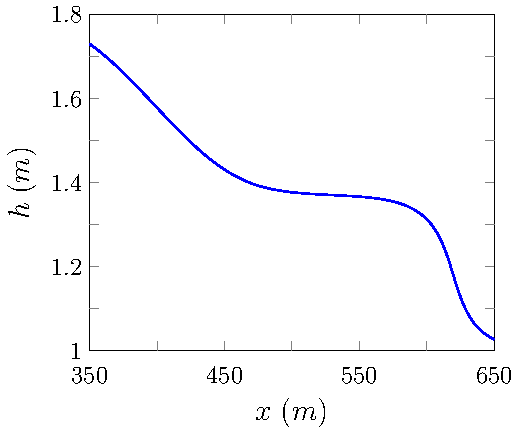
\includegraphics[width=\textwidth]{./chp2/figures/DamBreakStruct/1.pdf}
		\subcaption{Non-oscillatory Structure}
		\vspace{0.5cm}
	\end{subfigure}%
	\begin{subfigure}{0.5\textwidth}
		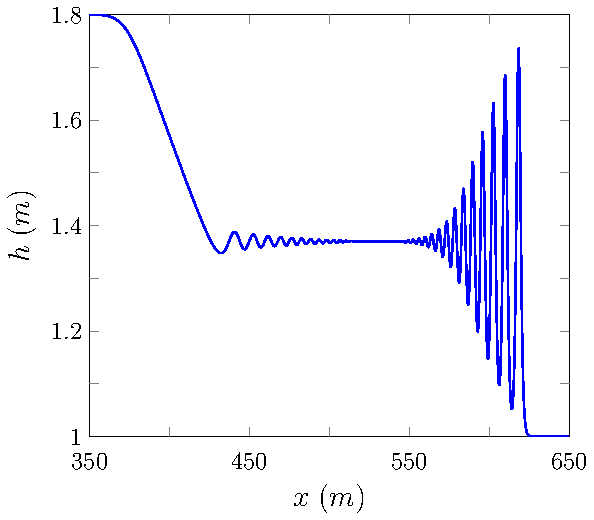
\includegraphics[width=\textwidth]{./chp2/figures/DamBreakStruct/6.pdf}
		\subcaption{Flat Structure}
		\vspace{0.5cm}
	\end{subfigure}
	\begin{subfigure}{0.5\textwidth}
		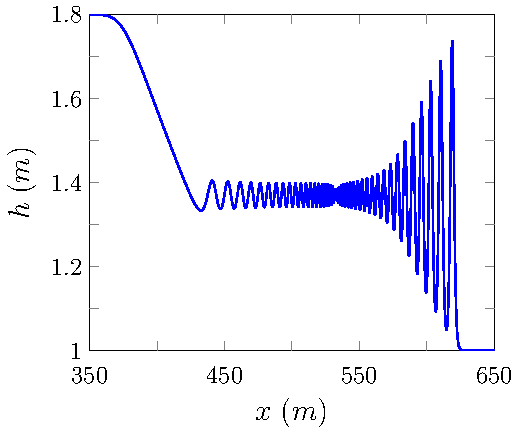
\includegraphics[width=\textwidth]{./chp2/figures/DamBreakStruct/9.pdf}
		\subcaption{Node Structure}
		\vspace{0.5cm}
	\end{subfigure}%
	\begin{subfigure}{0.5\textwidth}
		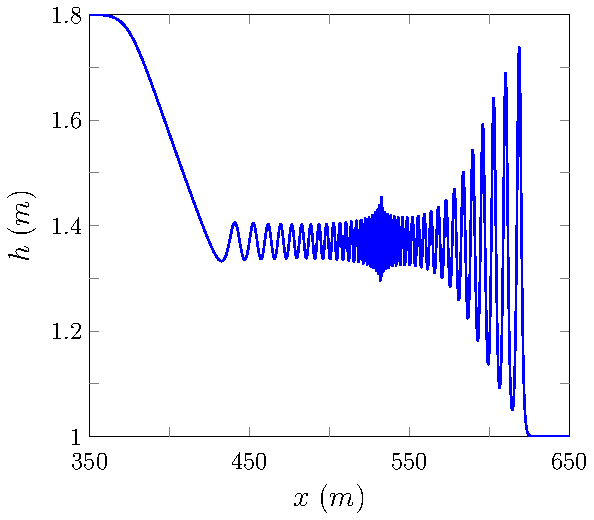
\includegraphics[width=\textwidth]{./chp2/figures/DamBreakStruct/20.pdf}
		\subcaption{Growth Structure}
		\vspace{0.5cm}
	\end{subfigure}
	\caption{Comparison of the different structures observed in numerical solutions displayed by \citet{Pitt-2018-61}.}
	\label{fig:DBExAll}
\end{figure}

The growth structure was consistently observed in numerical solutions of the smoothed dam-break problem as $\alpha \rightarrow \infty$ from high-order accurate methods on high resolution grids and thus well represents the structure of the solution of the Serre equations for this dam-break problem at $t=30s$. For this particular dam-break problem, the observation of other behaviours at $t=30s$ is caused by; small $\alpha$ values which overly smooth the initial conditions, low-order numerical schemes introducing large diffusive errors and low numerical resolutions which cannot resolve the higher frequency waves observed in the growth structure. These structures exist on a spectrum  where the severity of these effects determine the observed behaviour. So that the most severe damping effects produced the non-oscillatory structure and the least severe effects produced the justified growth structure. These effects explained the observations of different structures previously present in the literature \cite{El-etal-2006,Hank-etal-2010-2034,Mitsotakis-etal-2014,Mitsotakis-etal-2017,doCarmo-etal-2018-404}. 

The differences in the observed structures are primarily driven by the different internal structures of the bore, so that for the flat, node and growth structure in Figure \ref{fig:DBExAll} the undulation at the front of these bores are essentially identical. Therefore, the results of numerical solutions that haven't resolved all the internal structure present in the growth structure still agree well with the Whitham modulation results \eqref{eqn:ELWhitMod} of \citet{El-etal-2006}.

The amplitude of waves at the centre of the growth structure decay over time, resulting in the observation of the flat structure  when $t$ is larger. Therefore, these results agree with the linear argument put forth by \citet{Dougalis-etal-2007} as $t$ becomes large. This indicates that for smaller times the nonlinear terms of the Serre equations play a significant role in the evolution of steep gradients, while for long times the linear terms are dominant and thus a separation of the dispersive wave trains is observed. 

